\section{Измерения}

\subsection{Условия проведения измерений}

\begin{itemize}
    \item \textbf{Модель ЦПУ:} Intel(R) Core(TM) i7-4700HQ CPU @ 2.40GHz
    \item \textbf{Операционная система:} Linux 3.13.0-24-generic
    \item \textbf{Браузеры:}
      \begin{itemize}
        \item Google Chrome 41.0.2272.89;
        \item Mozilla Firefox 36.0.1.
      \end{itemize}
\end{itemize}

Измерения производились с помощью сервиса jsperf\footnote{\url{http://jsperf.com/}}.

\subsection{Микробенчмарки}

По оси Y отложено количество операций в секунду (чем больше, тем лучше).

\begin{figure}[H]
  \begin{center}
    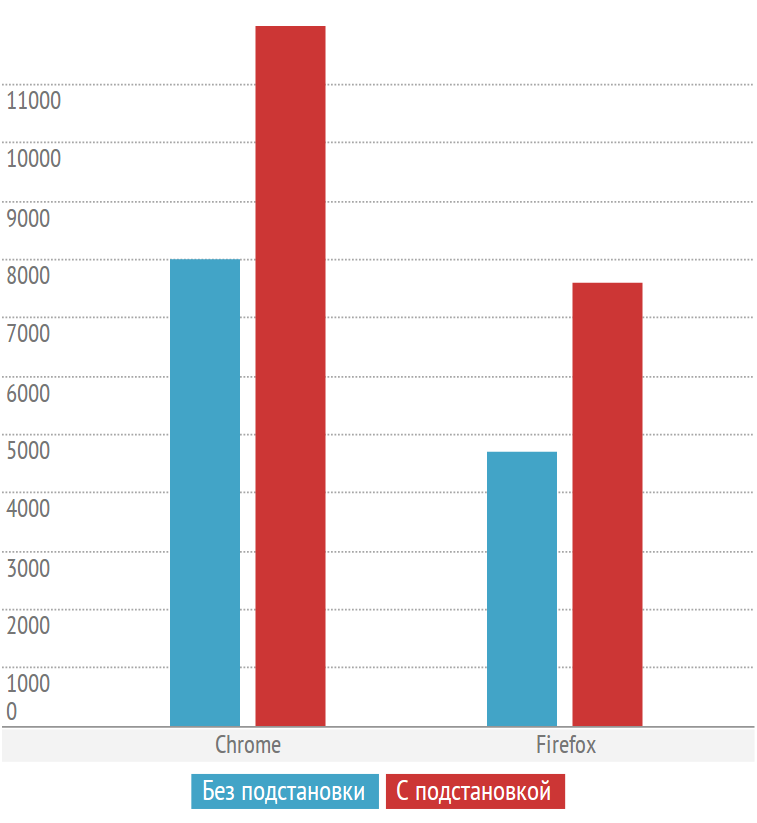
\includegraphics[scale=0.4]{benchmark-map}
  \end{center}
  \caption{Измерение вызова функции map}
\end{figure}

\begin{figure}[H]
  \begin{center}
    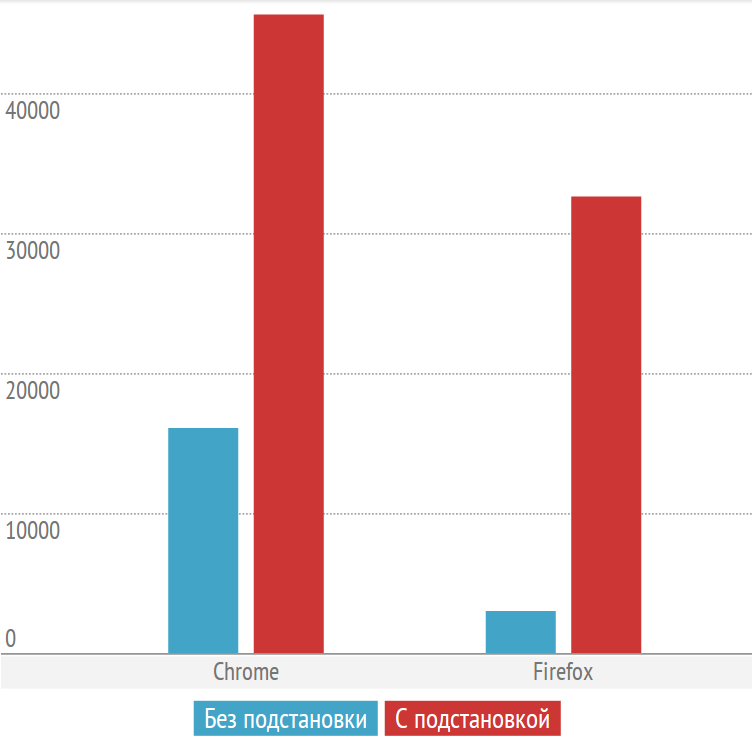
\includegraphics[scale=0.4]{benchmark-foreach}
  \end{center}
  \caption{Измерение вызова функции foreach}
\end{figure}
